\documentclass[
	% -- opções da classe memoir --
	12pt,				% tamanho da fonte	
	oneside,          % não imprimir em verso e anverso, oposto do twoside 
	a4paper,			% tamanho do papel. 
	% -- opções da classe abntex2 --
	chapter=TITLE,		% títulos de capítulos convertidos em letras maiúsculas
	section=TITLE,		% títulos de seções convertidos em letras maiúsculas
	subsection=TITLE,	% títulos de subseções convertidos em letras maiúsculas
	%subsubsection=TITLE,% títulos de subsubseções convertidos em letras maiúsculas
	% -- opções do pacote babel --
	english,			% idioma adicional para hifenização
	brazil			% o último idioma é o principal do documento
	,sumario=tradicional,
	]{abntex2-IFC}


% ---
% Pacotes fundamentais 
% ---
\usepackage{cmap}				% Mapear caracteres especiais no PDF
\usepackage{times}			    % Usa a fonte Times
\usepackage[T1]{fontenc}		% Selecao de codigos de fonte.fontenc
\usepackage[utf8]{inputenc}		% Codificacao do documento (conversão automática dos acentos)
\usepackage{lastpage}			% Usado pela Ficha catalográfica
\usepackage{indentfirst}		% Indenta o primeiro parágrafo de cada seção.
\usepackage{color}				% Controle das cores
\usepackage{graphicx}			% Inclusão de gráficos
\usepackage{amsfonts}			% Símbolos
%----Ajuste no alinhamento das listas
\usepackage{enumitem}
\setitemize[0]{itemindent=0.4cm,itemsep=0pt}
\setenumerate[0]{itemindent=0.5cm,itemsep=0pt}
%------
% ---
% Pacotes de citações
% ---
\usepackage[brazilian,hyperpageref]{backref}	 					  % Paginas com as citações na bibl

\usepackage[a4paper]{geometry}
%Referência
\usepackage[alf, 	
			 		abnt-emphasize=bf,
				    abnt-url-package=none,
				    abnt-repeated-title-omit=yes,
				    abnt-full-initials=yes,                                        %yes nome por extenso, no apenas iniciais
					abnt-etal-list=3												%abreviar com mais de 3 autores
]{abntex2/abntex2cite}				 														    % Citações padrão ABNT
\usepackage{lipsum}							   								       % para geração de dummy text
\usepackage{multirow}
\usepackage{float}
\usepackage{setspace}
\usepackage{tabularx}
\newcolumntype{b}{>{\hsize=2.3\hsize}X}
\newcolumntype{s}{>{\hsize=.45\hsize}X}
\newcolumntype{m}{>{\hsize=.9\hsize}X}

%\usepackage[none]{hyphenat}
%\captionsetup[table]{justification=raggedright}
% Configurações de aparência do PDF final
% alterando o aspecto da cor azul
\definecolor{blue}{RGB}{41,5,195}

% --- 
% Espaçamentos entre linhas e parágrafos 
% --- 
% O tamanho do parágrafo é dado por:
\setlength{\parindent}{2cm}
\linespread{1.5}

%Espaçamento depois dos títulos
\setlength{\afterchapskip}{\baselineskip}
% %\setlength{\afterchapskip}{\lineskip}

% Controle do espaçamento entre um parágrafo e outro:
\setlength{\parskip}{0cm}  % tente também \onelineskip

\hangcaption
\captionstyle[\raggedright]{}

%Estava mostrando nas referencias quais paginas estavam sendo referenciadas
\renewcommand{\backref}{}
\renewcommand*{\backrefalt}[4]{}

%Reduzir a fonte do caption
%\captionnamefont{\centering\ABNTEXfontereduzida}
%\captiontitlefont{\centering\ABNTEXfontereduzida}
%Ajuste nas listas de tabela, ilustrações e quadros
\setlength\cftbeforechapterskip{0pt}
% ---
% compila o indice
% ---
\makeindex
% ---

%----Include da capa é fora do documento 
% ---
% Informações de dados para CAPA e FOLHA DE ROSTO
% ---

\titulo{\uppercase{Balanceamento de Carga com CORBA e Docker}}
\autor{\uppercase{Leandro Ramos Marcelino}}
\local{Rio do Sul}
\data{2018}
\orientador[Orientadora:]{María Elena Villarreal, MEsc}
\instituicao{Ministério da Educação\\
        Secretaria de Educação Profissional e Tecnológica\\
        Instituto Federal Catarinense\\
        Campus Rio do Sul}
\tipotrabalho{Trabalho de Conclusão de Curso}
% O preambulo deve conter o tipo do trabalho, o objetivo, 
% o nome da instituição e a área de concentração
\preambulo{Trabalho de Conclusão de Curso apresentado ao
Curso de graduação em Ciência da Computação do
Instituto Federal Catarinense – Campus Rio do Sul para
obtenção do título de bacharel em Ciência da Computação.

Orientador: \imprimirorientador
}
% ---


%---

\begin{document}
% Retira espaço extra obsoleto entre as frases.
\frenchspacing 

% ----------------------------------------------------------
% ELEMENTOS PRÉ-TEXTUAIS
% ----------------------------------------------------------

%--- CAPA ----
\imprimircapa

% --- FOLHA DE ROSTO
\imprimirfolhaderosto
% \imprimirfolhaderosto* (o * indica que haverá a ficha bibliográfica)

% Inserir FOLHA DE APROVAÇÃO
\begin{folhadeaprovacao}

  \begin{center}
  \vspace*{-1.2cm}
    \textbf{\large\imprimirautor}
    
    \vspace*{\fill}\vspace*{\fill}\vspace*{\fill}
    \parbox{15cm}{
        \OnehalfSpacing\centering\large\textbf{\imprimirtitulo}
    }
    \vspace*{\fill}\vspace*{\fill}
    
    \hspace{.45\textwidth}
    \begin{minipage}{.5\textwidth}
        Este Trabalho de Curso foi julgado
        adequado para a obtenção do título de
        Bacharel em Ciência da Computação e
        aprovado em sua forma final pelo curso de
        graduação em Ciência da Computação do Instituto Federal Catarinense
        – Campus Rio do Sul. 

    \end{minipage}%
    \vspace*{\fill}
   \end{center}
    \vspace{-1cm}
  \begin{center}
  	 Rio do Sul (SC), dia de mês de ano
  \end{center}
  

    %\vspace{-1cm}

  
   \assinatura{\begin{center}\vspace{-0.7cm}\imprimirorientador \\ 
   					   Instituto Federal Catarinense – Campus Rio do Sul
   					   \end{center}
   			  }
   			  
    \begin{center}
  	\textbf{ BANCA EXAMINADORA}
   \end{center}
   %\vspace{-1cm}
   \assinatura{\begin{center}\vspace{-0.7cm}Definir\\ 
   					   Instituto Federal Catarinense – Campus Rio do Sul
   					     \end{center}
   }
    \assinatura{\begin{center}\vspace{-0.7cm}Definir \\ 
   					    Instituto Federal Catarinense – Campus Rio do Sul
   					    \end{center}
    }
    

    \vspace*{1cm}
  
\end{folhadeaprovacao}

% Inserir FOLHA DE AUTORIZAÇÃO
%\chapter{folhadeautorizacao}

  \begin{center}
  \vspace*{1 cm}
  \vspace{-2cm}
   \centering
\includegraphics[width=1.5cm]{brasaoRepublicaPeB.jpg}
   \vspace{-0.5 cm}
    {\large \SingleSpacing \imprimirinstituicao}
    \vspace{-0.5cm}
    \center{ \hrulefill}
    
     {\large \SingleSpacing \textbf{Autorização}}
    
    
    \vspace*{1 cm}
    
    \raggedleft{ Videira (SC), 19 de Novembro de 2016}
    \vspace*{0.5 cm}
    
   \end{center}
   


Eu, NOME SOBRENOME, regularmente matriculado na disciplina de Trabalho de Conclusão de Curso II - TC II do curso de Bacharel em Ciência da Computação, sob matrícula nº. XXXXXXX, pelo presente documento, autorizo o Instituto Federal Catarinense - IFC-Câmpus Videira, a utilizar o meu TC II intitulado "\imprimirtitulo", sob a orientação d Professor \imprimirorientador, para futuras informações e divulgações promovidas pelo Curso, e pelo Instituto, de forma institucional, em todo território nacional e internacional, sem fins comerciais, por qualquer meio de comunicação, tornando-o acessível a qualquer pessoa com interesse no trabalho.

A presente autorização substancia um consentimento de vontade e isenta de qualquer vício, feito de forma gratuita, e no gozo da minha capacidade civil, pelo que declaro nada me ser devido pelo curso de Ciência da Computação e pelo IFC-Câmpus Videira, ou seus representantes, em tempo algum, seja que título for, no que se refere, direta ou indiretamente, ao presente consentimento de uso da minha imagem e meu trabalho.

Declaro, ainda, que a utilização de meu nome e de meu trabalho, não constitui ofensa ou violação de meus direitos, nos termos do inciso X, do artigo 5o. da Constituição Federal.

Pelo presente também declaro ser de minha total responsabilidade o conteúdo de meu trabalho de conclusão de curso, descrito neste documento.

Os direitos e as obrigações aqui avençados transmitem-se aos meus herdeiros e sucessores.



  
   
   \vspace*{\fill}
   \vspace{-0.5 cm}
   
   \noindent Nome: \imprimirautor
   
   \vspace{0.25 cm}
   
   \noindent CPF: XXXXXXXXXXXXXX
   
   \vspace{0.25 cm}
   
   \noindent Assinatura: \hskip-3em\vtop{\vskip.05cm\hsize=5in \hrulefill}
   
   \vspace{0.5 cm}
   
    \begin{center}
    Rod. SC 135, KM 125 - Campo Experimental - CEP: 89560-000 - Videira - SC \\
    Fone: (49) 3533-4900 - http://www.ifc-videira.edu.br
    \end{center}

    \vspace*{1cm}


% DEDICATÓRIA
%\begin{dedicatoria}
 \vspace*{\fill}
 \noindent
  \raggedleft
 \begin{minipage}{.54\textwidth}
    Dedico este trabalho ...
   \end{minipage}
\end{dedicatoria}


% AGRADECIMENTO
%\begin{agradecimentos}

agradecimentos

\end{agradecimentos}

%EPÍGRAFE
%\include{pretextuais/epigrafe}

% RESUMO
%% resumo em português
\begin{resumo}
\noindent
 
Neste trabalho
 \vspace{0.2cm}   
Palavras-chave: palavra 1. palavra 2. palavra 3
 
\end{resumo}
 
% resumo em inglês
\begin{resumo}[Abstract]	
\begin{otherlanguage*}{english}
\noindent 
 
This is the abstract of this work.
 
\vspace{0.2cm}
Key-words: Word 1. Word 2. Word 3
\end{otherlanguage*}
\end{resumo}


% lista de ilustrações
\pdfbookmark[0]{\listfigurename}{lof}
\listoffigures*
\cleardoublepage
% ---

% lista de quadros
% --- 
%PRECISO VER COMO FAZER O CONTROLE DE QUANDO TIVER MENOS Q 10 VAI PARA LISTA DE ILUSTRAÇÕES
%\pdfbookmark[0]{\listofquadrosname}{loq}
%\listofquadros*
%\cleardoublepage
% ---

% LISTA DE TABELAS
\pdfbookmark[0]{\listtablename}{lot}
\listoftables*
\cleardoublepage  %-- força proxima pagina

% ---
% inserir lista de abreviaturas e siglas
% ---
%\begin{siglas}
%  \item[SIGLA] descrição

%\end{siglas}
% ---

% ---
% inserir lista de símbolos
% ---
%\begin{simbolos}
%  \item[$ \Gamma $] Descrever o que o símbolo representa em seu trabalho. Exemplo abaixo.
%  \item[$ \omega $] Frequência angular [rad/s].
%  \item[$ \zeta $] Coeficiente de amortecimento.

%\end{simbolos}
% ---

% SUMARIO
\pdfbookmark[0]{\contentsname}{toc}
\tableofcontents*
\cleardoublepage

% ------------------------------------------------------
% ELEMENTOS TEXTUAIS
% ------------------------------------------------------
\textual
% INTRODUÇÃO
\chapter{INTRODUÇÃO}
	Os computadores e seus sistemas mudando e evoluindo constantemente, começando em 1945 até 1985 onde eram extremamente grandes e caros, avançando para computadores com microprocessadores de 8, 16, 32, 64 bits e drasticamente compactos, tornando muito mais acessíveis as empresas.
	
	Outra evolução que fez total diferença foi o surgimento das redes de computadores de alta velocidade, desde redes locais (LANs) a redes de longa distância (WANs), que permitiram que máquinas de computadores pudessem trocar mensagens e conversar.
	
	A computação evoluiu muito, os processadores começaram a ter mais núcleos para aumentar seu poder de processamento com o paralelismo de tarefas, porém um limite foi alcançado e para superá-lo a solução foi dividir para conquistar, sistemas compostos por vários computadores interligados foram criados para aumentar ainda mais o poder computacional, estes sistemas ficaram conhecidos como sistemas distribuídos.
	
	Um sistema distribuído consiste em um conjunto de componentes de \textit{softwares} e/ou \textit{hardwares} conectados em uma rede de computadores que são capazes de organizar suas ações somente pela troca de mensagens \cite{Coulouris-2012}. Desta forma, processos são executados simultaneamente em máquinas diferentes, o que aumenta a velocidade do sistema, além de outros fatores como segurança, tolerância a falha, disponibilidade e confiabilidade.
	
	Assim como o poder de processamento e a comunicação em redes evoluíram, a virtualização de computadores também. Computadores são passíveis de falha, e substituir uma máquina pode ser extremamente trabalhoso, refazer todas as configurações e alcançar o mesmo estado de uma outra máquina é uma quase uma missão impossível. Manter diversas máquinas ligadas ao mesmo tempo pode ser muito custoso, pela manutenção e inclusive pela possibilidade de haver recursos sobrando que poderiam estar sendo melhor utilizados.
	
	A virtualização de computadores surgiu para sanar alguns destes problemas, uma máquina poderia fazer o papel de múltiplas, com heterogeneidade de sistemas operacionais e configurações, além de facilitar sua manutenção, porque todo o sistema e suas configurações ficavam salvas e poderiam ser transportadas ou copiadas para uma nova máquina a qualquer momento.
	
	Visto que a virtualização para sistemas distribuídos era vantajosa, este âmbito também evoluiu. Simular todo um sistema operacional pode custar muito caro pois existe desperdício de tempo com processos desnecessários, surgiu então a era dos \textit{containers}. Estes são ambientes de execução criados para um programa específico, criando um ambiente computacional somente com o necessário para sua execução, tornando sua execução muito mais rápida e segura.
	
\section{PROBLEMATIZAÇÃO}
	Sistemas distribuídos são executados em múltiplas máquinas e portanto podem apresentar falha parcial, onde um dos componentes apresenta problemas enquanto os outros continuam funcionando normalmente. Alguns componentes podem ser afetados por esta falha e outros não, porém de forma alguma o sistema como um todo pode parar de executar, ele deve ser capaz de tolerar este problema e recuperar-se do mesmo.
	
	Há forte relação entre ser tolerante a falha e os denominados sistemas confiáveis \cite{Tanenbaum}. Ao planejar um sistema distribuído os seguintes requisitos devem ser levantados: Disponibilidade, Confiabilidade e Segurança. Em outras palavras deve ficar garantido que o sistema poderá ser utilizado a qualquer momento, que este trará respostas corretas e que deverá executar todos os procedimentos sem apresentar falhas para o usuário final.
	
\subsection{Solução proposta}
	Manter um sistema disponível a todo instante é complexo pois várias falhas podem acontecer, diferentes cargas de processamento podem ser requeridas e este não pode parar por falta de recursos, outros componentes também não poderão ser afetados. A capacidade de aumentar ou reduzir seus recursos conforme utilização e de multiplicar a quantidade de componentes para suprir a demanda deve ser rápida e eficaz.

	A finalidade deste trabalho será construir um sistema distribuído que utilizará \textit{microcontainers} e será composto por múltiplos componentes, com diferentes atribuições e sistemas operacionais, que seja capaz de apresentar os pilares da disponibilidade e confiabilidade a partir da utilização do balanceamento de carga. O sistema deve estar disponível a todo tempo, sendo capaz de migrar seus componentes de forma rápida e transparente ao usuário.
	
\subsection{Delimitação do escopo}
	O trabalho tem como objetivo desenvolver uma aplicação simples em um sistema distribuído criado por \textit{microcontainers} que seja capaz de apresentar os conceitos da disponibilidade e confiabilidade com balanceamento de carga, realizando migrações rápidas e transparentes. Para alcançar os objetivos serão utilizados \textit{microcontainers} com Docker, o sistema será desenvolvido com a linguagem de programação Java e para comunicação entre os componentes o \textit{middleware} CORBA.
	
\subsection{Justificativa}
	A replicação de dados é extremamente importante para tornar o sistema mais confiável e aumentar seu desempenho. Se um sistema de arquivos foi replicado, pode ser possível continuar trabalhando após a queda de uma réplica simplesmente com a comutação para uma das réplicas \cite{Tanenbaum}. Sistemas distribuídos devem também ser capazes de se recuperar automaticamente de falhas parciais sem afetar o restante dos processos.
	
	Neste contexto uma aplicação capaz de executar seus processos mesmo na presença de falhas, e que supra a demanda de requisições do cliente é aceitável e eficaz para o conceito de balanceamento de carga. Sendo sua estrutura e construção um forte exemplo para a criação de aplicações mais complexas com disponibilidade e confiabilidade.
	
\section{OBJETIVOS}
\subsection{Objetivo Geral}
	Desenvolver uma estrutura com \textit{microcontainers} que aplique os conceitos de disponibilidade e confiabilidade utilizando o balanceamento de carga em um sistema de controle financeiro pessoal.
	
\subsection{Objetivos Específicos} 
\begin{enumerate}[label=\alph*]
	\item Desenvolver uma aplicação simples com interface web, regras de negócio e persistência separados em componentes diferentes;
	\item Criar estrutura com \textit{microcontainers} que execute a aplicação;
	\item Aplicar os conceitos de disponibilidade em sistemas distribuídos;
	\item Aplicar os conceitos de confiabilidade em sistemas distribuídos;
	\item Utilizar balanceamento de carga, com migração rápida e transparente;
	\item Realizar testes com alta demanda de clientes e também com falhas forçadas para validar que o sistema é capaz de superar os obstáculos e confirmar que os conceitos aplicados funcionam.
\end{enumerate}

\section{METODOLOGIA}
	escrever aqui

\begin{enumerate}
	\item Revisão Bibliográfica: O trabalho será fundamentado através de orientação profissional e pesquisa em livros, artigos publicados, trabalhos correlatos e monografias sobre Sistemas Distribuídos, CORBA e Docker;
	\item Estudo sobre Sistemas Distribuídos: Estudo dos fundamentos de sistemas distribuídos, principais conceitos, objetivos e atributos necessários para o desenvolvimento do trabalho;
	\item Estudo sobre CORBA: Estudo dos principais métodos e configurações necessárias para alcançar o objetivo do trabalho;
	\item Estudo sobre Docker: Estudo sobre seus conceitos e utilização, desde conceitos básicos até formas avançadas de orquestrar vários \textit{containers};
	\item Modelagem: Modelagem do sistema através de Diagrama de \textit{Deployment}, Diagrama de Classes e Diagrama de Sequência, tem por finalidade complementar o primeiro objetivo específico.
	\item Desenvolvimento: Para o desenvolvimento do projeto será utilizado a linguagem de programação Java, o \textit{middleware} CORBA e \textit{microcontainers} Docker.
	\item Fase de testes: Esta fase consiste em simular uma alta demanda do sistema que deve ser capaz de replicar-se e ser consistente. A simulação de falhas também será necessária para demonstrar que o sistema é capaz de continuar executando até ser corrigido.
\end{enumerate}

%FUNDAMENTAÇÃO TEORICA
\chapter{FUNDAMENTAÇÃO TEÓRICA}

Neste capítulo serão abordados conceitos relacionados a Sistemas Distribuídos e os recursos necessários para realizar balanceamento de carga, tendo forte embasamento nos autores \citeauthoronline{Tanenbaum} e \citeauthoronline{Coulouris-2012} que são de grande renome no âmbito de sistemas distribuídos.

\section{Sistemas Distribuídos}
	%Introduzir as definições explicando que vou utilizar de dois autores, blablabal

	Graças aos grandes avanços tecnológicos no decorrer dos últimos 50 anos, tornou-se possível criar sistemas compostos por inúmeros computadores ligados por uma rede de alta velocidade, também conhecidos como sistemas distribuídos. Estes podem ser definidos como um conjunto de computadores independentes que se apresenta a seus usuários como um sistema único e coerente \cite{Tanenbaum}.
	
	Segundo \citeauthoronline{Coulouris-2012} (\citeyear{Coulouris-2012}) um sistema distribuído consiste em um conjunto de componentes de \textit{softwares} e/ou \textit{hardwares} conectados em uma rede de computadores que são capazes de organizar suas ações somente pela troca de mensagens.
	
	Sistemas distribuídos são então, um conjunto de componentes computacionais independentes conectados por uma rede em que, a partir da troca de mensagens, representam um único sistema para o usuário final.
	
	Os computadores e programas que compõem um sistema são autônomos e se apresentam aos usuários ou programas como um sistema único, o que implica na colaboração entre eles, a forma como ela se estabelece é a questão mais importante do sistema \cite{Tanenbaum}. 
	
	Uma característica forte nos sistemas distribuídos é ser heterogêneo, ou seja, ser composto por diferentes \textit{hardwares}, sistemas operacionais e \textit{softwares} de variadas linguagens de programação. Estas diferenças e a forma de comunicação entre elas é oculta ao usuário. Expandir a quantidade de máquinas também deverá ser possível, sendo que cada máquina é autônoma, isto serve principalmente para que a aplicação possa continuar executando mesmo com algum computador avariado \cite{Tanenbaum}.
	
	A transparência do sistema, ou seja, ocultar que os recursos e processos estão ocorrendo em máquinas diferentes é uma das principais metas dos sistemas distribuídos. Este conceito está ligado a diversos aspectos do sistema, podendo ser resumido nas transparências apresentadas na tabela \ref{transparencia}.
	
	\begin{table}[]
		\caption{Formas de transparência em sistemas distribuídos.}
		\label{transparencia}
		\fonte{
			\citeauthoronline{Tanenbaum} 
			\citeyear{Tanenbaum}
		}
		\begin{tabularx}{\linewidth}{|l|m|}
			\hline
			\textbf{Transparência} & \textbf{Descrição} \\ \hline
			Acesso & Oculta diferenças na representação de dados e no modo de acesso a um recurso \\ \hline
			Localização & Oculta o lugar em que um recurso está localizado \\ \hline
			Migração & Oculta que um recurso pode ser movido para outra localização \\ \hline
			Relocação & Oculta que um recurso pode ser movido para uma outra localização enquanto em uso \\ \hline
			Replicação & Oculta que um recurso é replicado \\ \hline
			Concorrência & Oculta que um recurso pode ser compartilhado por diversos usuários concorrentes \\ \hline
			Falha & Oculta a falha e a recuperação de um recurso \\ \hline
		\end{tabularx}
	\end{table}
	
	No trabalho serão abordados principalmente dois conceitos, transparência de acesso que oculta as diferenças de arquitetura das máquinas, fazendo com que sistemas operacionais diferentes possam se comunicar de forma padrão e tornem suas diferenças imperceptíveis. E transparência de localização que faz com que o usuário desconheça o local físico em que um recurso se encontra. 
	
	Uma das formas de obter transparência e então fazer a conexão entre as máquinas de diferentes sistemas operacionais, aplicações e localizações em um sistema único, é a partir do uso de \textit{middlewares}. 
	
	\subsection{Middleware}
	O termo \textit{middleware} está relacionado a uma camada de \textit{software} que torna possível a programação abstrata e mascarar as diferenças de \textit{hardware}, sistema operacional e linguagens de programação dos componentes que fazem parte do sistema distribuído. Cada \textit{middleware} tem suas próprias características, alguns suportam apenas uma linguagem de programação, invocação de objetos ou eventos remotamente, entre outras \cite{Coulouris-2012}.
	
	O \textit{middleware} é representado por processos ou objetos em um conjunto de computadores que se comunicam e compartilham recursos para aplicações distribuídas \cite{Coulouris-2012}. A Figura \ref{fig:Tanenbaum-middleware} apresenta quatro máquinas autônomas que são responsáveis por aplicações somente suas ou compartilhadas, a comunicação entre estas máquinas heterogêneas é coordenada pelo \textit{middleware}. 
		
	\begin{figure}[htb]
		\caption{Atuação da camada \textit{middleware}}
		{\parbox{6cm}{
				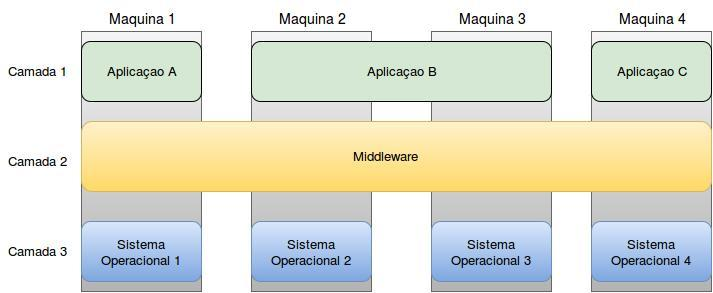
\includegraphics[width=14cm]{images/middleware.jpeg}
				\label{fig:Tanenbaum-middleware}
				\fonte{
					\citeauthoronline{Tanenbaum} 
					\citeyear{Tanenbaum}
				}
		}}
	\end{figure}

	Sistemas de \textit{middleware} costumam seguir um estilo arquitetônico específico, CORBA segue um estilo baseado em objetos, enquanto TIB/Rendezvous foi desenvolvido para arquitetura baseadas em evento. Usar uma arquitetura específica como molde simplifica o projeto de aplicações.
	
	A orientação a objetos é um conceito forte no desenvolvimento de \textit{software} e foi utilizado para a criação de sistemas baseados em objetos distribuídos. Um objeto tem como característica o encapsulamento de dados e operações que podem ser utilizadas, nos sistemas um cliente costuma ter somente uma interface que é a declaração das operações que podem ser executadas, enquanto o servidor guarda os objetos com a implementação das interfaces, os objetos. O servidor também contém um esqueleto, que fornece o mínimo necessário de meios para que o \textit{middleware} acesse os objetos.
	
	Os objetos em sistemas distribuídos existem em vários formatos, sendo comum serem similares a objetos de linguagens de programação como C ou Java. Entre os principais \textit{middlewares} que aderiram esta ideia está o CORBA, alvo do desenvolvimento deste trabalho.
	
	%Apresentar alguns middlewares (RMI, Rest, CORBA) e fazer um gancho para CORBA
\section{CORBA}
	O CORBA (\textit{Common Object Request Broker Architecture}) é uma arquitetura com a finalidade de permitir que objetos de sistemas distribuídos possam se comunicar de forma transparente entre si, sem depender de suas plataformas de hardware, sistemas operacionais e linguagem de programação na qual foram desenvolvidos. Por este motivo, a arquitetura está entre as melhores opções para desenvolver aplicações de interação cliente/servidor (RICCIONI, 2003).
	
	O modelo tem como base três conceitos principais: integração e reuso de componentes, orientação a objetos e um ambiente de computação distribuído e aberto. A arquitetura CORBA utiliza o modelo cliente/servidor e também um mediador entre estes agentes visando reduzir a complexidade de sua interação. O mediador é conhecido como ORB (\textit{Object Request Broker}) e é responsável por localizar os objetos para qual se destinam as requisições da rede, além do envio dos parâmetros da requisição e de suas respectivas respostas, caso existam.

	CORBA é uma arquitetura que permite a interação entre objetos distribuídos em diferentes linguagens e sistemas, além de proporcionar maior transparência na comunicação entre os objetos. Para localizar os objetos são feitas referências que poderão ser resolvidas pelo ORB.
	
	Para descrever as interfaces dos objetos é utilizada a linguagem IDL (\textit{Interface Definition Language}), esta é uma linguagem que contém apenas declarações. Os tipos de dados são exclusivos da linguagem e são mapeados para tipos respectivos de acordo com as linguagens que ela suporta.
	
	Em um arquivo .idl é possível definir um módulo que conterá todas as outras definições: tipos de dados, estruturas de dados, métodos, parâmetros e exceções. A partir deste arquivo é possível criar diversas interfaces com diferentes compiladores para diferentes linguagens.
	
	Uma vez que os arquivos java são gerados, é necessário que você implemente os métodos e exceções para que eles funcionem da forma desejada. Após implementar basta ambos servidor e  cliente utilizarem os objetos ORB para fazer a comunicação.

\section{Balanceamento de Carga}
	Diferente dos sistemas de máquina única, os sistemas distribuídos apresentam a possibilidade de falha parcial, ou seja, um dos componentes ter problemas enquanto os outros continuam estão trabalhando. Esta falha poderá afetar o processo de alguns componentes e de outros não, mas o projeto do sistema já deve prever esta possibilidade e ser construído de forma a manter-se funcionando até se recuperar automaticamente da falha.
	
	Tolerar falhas é um dos pontos mais importantes em sistemas distribuídos e segundo \citeauthoronline{Tanenbaum} (\citeyear{Tanenbaum}) "Há forte relação entre ser tolerante a falha e os denominados sistemas confiáveis". Para tal são alçados alguns requisitos: Disponibilidade, capacidade de um sistema estar pronto para uso a qualquer momento de forma imediata. Confiabilidade, capacidade de um sistema executar o máximo possível de tempo sem apresentar falhas. Segurança, ser capaz de assegurar que mesmo apresentando falhas nada de grave acontecerá. Capacidade de manutenção, facilidade com que as falhas no sistema são corrigidas automaticamente ou não.
	
	Sistemas apresentam defeitos quando não são capazes de fornecer aos usuários todos os serviços que deveriam. Erros podem ocorrer por diversos motivos, sendo suas causas conhecidas como falhas, tolerar elas significa que um sistema possa continuar funcionando mesmo na presença das mesmas. As falhas são classificadas como transientes quando acontecem uma vez e não se repetem mais, intermitentes se acontecem vez ou outra mas sem conhecimento do motivo ou permanentes quando continuam acontecendo até serem corrigidas.
	
	As falhas dentro de um sistema distribuído podem ser várias, podem ser no próprio componente ou no meio de transmissão visto que eles precisam se comunicar entre si. Para abstrair o conhecimento desta imensidão de possibilidades, pode-se classificar as falhas como queda, omissão de recebimento, omissão de envio, temporização, valor de resposta, transição de estado da resposta e arbitrárias.
	
	Uma das formas de tolerar falhas é ocultando, sendo redundância a principal técnica de ocultação de falhas. É possível realizar redundância por tempo que fará com que caso uma ação falhe seja executada novamente por um determinado tempo, redundância física onde novos componentes são adicionados para possibilitar que o sistema ignora o mal funcionamento de outro componente, e redundância de informação na qual alguns dados repetidos são adicionados a resposta para que esta possa ser recuperada em caso de falha na transmissão.
	
	Com isto foram criados os processos em grupos que tem seu funcionamento dado pela replicação de processos em grupos, ou seja, uma mesma funcionalidade do sistema é executada por todos os componentes de um conjunto e com as \textit{n} respostas geradas é possível tolerar e detectar falhas, pois se um falhar outro irá se encarregar de responder.
	
	Grupos de processos podem apresentar estruturas internas diferentes, grupos simples são os que todos os processos podem ser iguais e sem nenhum tomador de decisão, já os grupos hierárquicos tem um processo coordenador que organiza as tarefas e define qual processo irá executar cada tarefa. Ambos apresentam prós e contras, grupos simples continuam a funcionar normalmente com a queda de um dos membros mas as tomadas de decisões são mais complexas, já grupos hierárquicos tem facilidade na tomada de decisões mas são dependentes de um coordenador, se este falhar o grupo inteiro fica parado.
	
	Outro princípio fundamental é a segurança, que está fortemente relacionada com a confiabilidade. A segurança se apresenta como um dos tópicos mais complexos pela necessidade de estar presente em todo o sistema, uma única falha pode destruir toda a estrutura construída.
	
	É possível dividir a segurança em duas partes, a comunicação entre usuários ou processos e a autorização que assegura que um processo receba acesso somente aos recursos habilitados. Existem também quatro principais tipos de ameaças a segurança: interceptação ocorre quando um componente não autorizado consegue acesso a um serviço ou dados restritos, interrupção quando arquivos são corrompidos ou perdidos, modificação quando ocorre uma alteração não autorizada em dados e invenção quando são gerados dados  ou atividades adicionais que não deveriam existir.
	
	A utilização de canais seguros é essencial, estes irão fornecer os meios necessários para autenticar ambas as partes que estão se comunicando e também proteger as mensagens enviadas contra modificação e leitura de membros exteriores. Outro ponto é a utilização de apenas um criptossistema simétrico ou até combinar este com um sistema de chave pública, também conhecido como chave de sessão.
	
	O controle de acesso deve ser utilizado para que somente os processos com permissão tenham acesso aos recursos solicitados. Uma forma de implementar este controle é fazer que cada recurso mantenha uma lista com os processo que podem acessar, ou então emitir certificados para os processos indicando as permissões de cada um.
	
\section{Containers}
	A ideia de dividir processos e intercalar sua execução de forma a parecerem simultâneos, que é muito comum em programação \textit{multithread}, é aplicada na virtualização de recursos que tende a simular múltiplos ambientes de \textit{hardware} e \textit{software} em um única máquina.
	
	É comum que os sistemas distribuídos ofereçam uma das várias interfaces de programação de software de alto nível, a virtualização substitui uma interface já existente para simular o comportamento de outro sistema. A real necessidade de virtualizar sistemas surgiu quando o \textit{hardware} começou a evoluir rapidamente na década de 90, mas os \textit{softwares} e \textit{middlewares} não acompanhavam o mesmo ritmo, simular os ambientes antigos colaborou para que a compatibilidade de sistemas fossem mantidas nas novas máquinas enquanto os programas evoluíam.
	
	A virtualização também surgiu para facilitar a manutenção dos administradores de sistemas, porque todo o sistema e suas configurações ficam salvas e podem ser transportadas ou copiadas para uma nova máquina a qualquer momento.
	
	A partir das grandes vantagens em se utilizar virtualização para sistemas distribuídos, junto a rápidas evoluções de \textit{hardware} e redes de computador, tornou-se possível evoluir também na forma de virtualizar. Simular todo um sistema operacional pode custar caro pois muito tempo e processamento são desperdiçados com processos desnecessários, com este cenário surge a era dos \textit{containers}.
	
	\textit{Containers} são ambientes de execução criados para um programa específico, isolando o mesmo de todos os recursos do computador que não serão necessários para seu funcionamento. Os principais benefícios são a segurança por remover o acesso a recursos desnecessários, rápida execução por não precisar iniciar grande parte dos componentes de um sistema operacional e tornar o programa executável em qualquer computador por garantir que este sempre estará executando em um mesmo ambiente computacional.

	Diferente das máquinas virtuais os \textit{containers} não utilizam virtualização de \textit{hardware}, os programas se comunicam diretamente com o \textit{kernel} do Linux da máquina. Isso porque não são adicionadas camadas extras entre o \textit{container} e o sistema operacional para ganhar desempenho ao não desperdiçar recursos simulando um ambiente de \textit{hardware}, conforme apresentado na Figura \ref{fig:Docker-container-vm}.

	\begin{figure}[htb]
		\caption{Diferença de camadas entre \textit{containers} e máquinas virtuais}
		{\parbox{6cm}{
				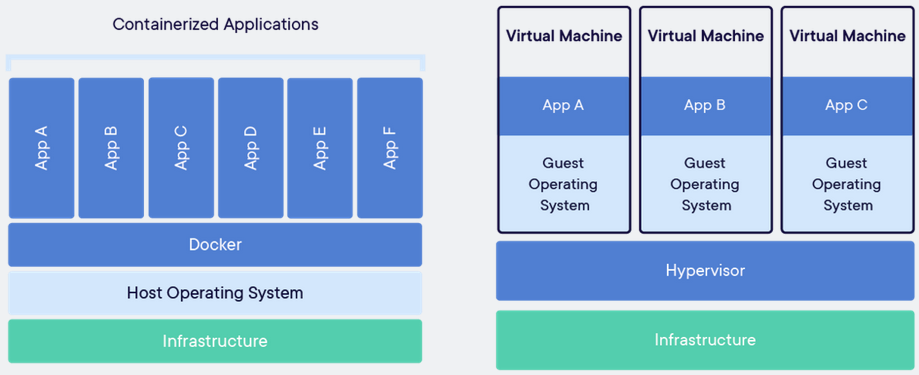
\includegraphics[width=15cm]{images/container_x_vm.png}
				\label{fig:Docker-container-vm}
				\fonte{
					https://www.docker.com/resources/what-container
					\citeyear{}
				}
		}}
	\end{figure}

	Apesar das vantagens apresentadas, a construção manual de um \textit{container} pode ser complexa e portanto pode ser feita da forma incorreta, com erros de configuração e falhas de segurança. Para facilitar e padronizar a construção destes surgiu o Docker, que a partir de configurações próprias cria um \textit{container} dentro dos padrões e utilizando as melhores práticas de construção.
	%Ligar com o tema de SD, mobilidade de aplicação, transparência e etc.
\subsection{Docker}
	De uma forma simples é possível definir Docker como uma maneira de abranger diferentes serviços em ambientes isolados, que contém todos os recursos necessários para garantir ao desenvolvedor que o serviço irá funcionar em qualquer local que o Docker seja executado \cite{Hane}.
	
	Docker desenvolveu sua própria ferramenta de construção de \textit{containers}. Ao ser instalado, disponibiliza uma interface de linha de comando que se comunica com um \textit{daemon} próprio, este é o responsável por organizar todas as instâncias em execução. Sendo assim, é considerado como um sistema para interagir com \textit{containers} no formato cliente-servidor, onde o terminal de comandos é o cliente e o \textit{daemon} é o servidor. Na figura \ref{fig:Docker-daemon} está apresentado uma estrutura executando Docker, que por sua vez está com três instâncias simultâneas com suas próprias dependências, executando de forma isolada.
	
	\begin{figure}[htb]
		\caption{Execução de \textit{containers} utilizando Docker em um sistema operacional Linux comum}
		{\parbox{6cm}{
				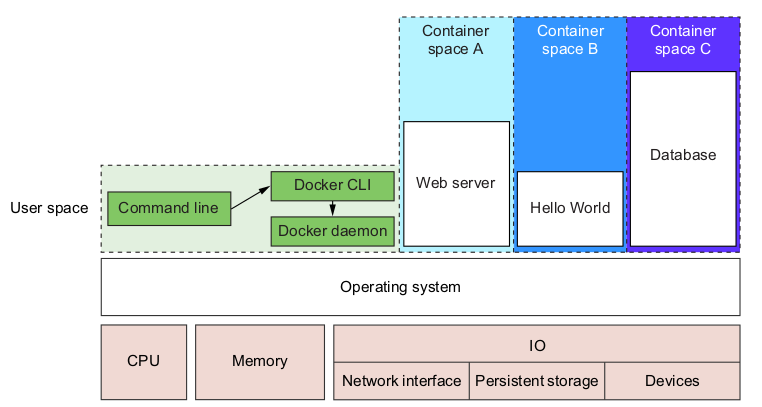
\includegraphics[width=15cm]{images/docker-daemon.png}
				\label{fig:Docker-daemon}
				\fonte{https://www.docker.com/resources/what-container}
		}}
	\end{figure}

O diferencial que o fez ganhar grande espaço no universo da tecnologia são as Imagens Docker, responsáveis por inicializar um \textit{container}. A imagem é um conjunto de instruções que define como deve ocorrer a criação do \textit{container} Docker, especificando qual ambiente computacional, bibliotecas e pacotes devem ser instalados, comandos a serem executados, configurações de memória, processamento, rede, assim como a criação de espaços de armazenamento próprio ou compartilhado. Com elas o processo de reprodução e distribuição de um \textit{container} que era complexo se torna simples, ainda mais com o repositório de imagens (DockerHub) mantido pela empresa, onde qualquer usuário pode fazer \textit{upload} e \textit{download} de imagens.





%TRABALHOS CORRELATOS
\chapter{TRABALHOS CORRELATOS}

\section{Fast Transparent Migration for Virtual Machines}
	Este trabalho apresenta um modelo de implementação de sistema utilizando máquinas virtuais para realizar migrações de forma rápida e transparente. Foi o primeiro a conseguir migrar sistemas sem nenhuma modificação e sem modificações no sistema operacional, funcionando para Windows, Linux e outros. A migração ocorre com total transparência, sem que nem os clientes e nem a aplicação consiga saber que o local de execução foi alterado.
	
	Sistemas com grande demanda podem apresentar lentidão ou falha nos serviços que prestam devido a falta de recursos na máquina em que o processamento está ocorrendo. A migração rápida e transparente é capaz de melhorar a utilização do serviço com o balanceamento de carga, movendo serviços para máquinas com mais recursos livres.
	
	O artigo descreve com um exemplo como foi capaz de viabilizar a migração transparente de sistemas com máquinas virtuais, sem a necessidade de efetuar alterações no programa ou no sistema operacional. Foram utilizadas medidas de desempenho de centenas de migrações de máquinas virtuais que utilizam padrões industriais de \textit{benchmark}, uo seja, os padrões mais utilizados na indústria de \textit{software}. Também descreve as necessidades de desempenho e recursos durante a migração.
	
	Para executar a migração inicialmente é selecionado a máquina virtual que será migrada e qual seu destino, uma cópia do estado atual da memória da máquina é copiado para o destino enquanto o serviço continua rodando em sua origem, em seguida o estado da máquina virtual é enviado também para finalizar a configuração do novo local. Uma vez que o destino está configurado ele começa a ser executado e o controle da máquina virtual é direcionado ao novo ambiente, para então enviar qualquer resto de estado de memória da máquina origem e removê-la de funcionamento.
	
	A utilização de máquinas virtuais foi essencial para o objetivo do artigo, a migração de aplicações era falha pela dificuldade em encapsular o estado de execução e também de manter as configurações do sistema operacional, ambos solucionados com a utilização de máquinas virtuais. A migração da memória física é o fator essencial para alcançar a transparência, apesar de tornar o processo mais lento ela faz com que a aplicação fique menos tempo fora do ar, menos de um segundo de acordo com os testes.
	
\section{LOAD BALANCING ALGORITHM TO IMPROVE RESPONSE TIME ON CLOUD COMPUTING}
	Balanceamento de carga na nuvem está relacionado a alocação de recursos computacionais para máquinas virtuais de forma que as aplicações ali executadas não falhem por falta de recursos e evitando lentidão para o cliente. A melhor prática para realizar o balanceamento de carga na nuvem irá depender da requisição efetuada que pode ser SaaS (\textit{Software as a Service}), PaaS (\textit{Platform as a Service}) ou IaaS (\textit{Infrastructure as a Service}).
	
	Este artigo propôs um algoritmo de balanceamento de carga para máquinas virtuais que busca aumentar o tempo médio de resposta e o tempo médio de processamento dos sistemas na nuvem, o algoritmo foi comparado aos já conhecidos algoritmos Maxmin, \textit{Throttled} e \textit{Avoid Deadlocks} para avaliar os resultados.
	
	Algoritmos dos autores Rashmi, Rajwinder e Hafiz foram utilizados como base de conhecimento, estes já buscavam otimizar o tempo médio de resposta e processamento no balanceamento de carga em máquinas virtuais. 
	
	A máquina virtual com maior disponibilidade e velocidade para completar a tarefa será selecionada a partir de certo parâmetros: lista da carga de trabalho do sistema, lista de tarefas já submetidas a execução, percentual já utilizado da máquina e o tempo de execução esperado virtual. 
	
	Os testes foram realizados com trinta tarefas a serem executadas, uma central de dados e três máquinas virtuais. Comparando ao algoritmo Throttled os tempos médios de execução e resposta foram inferiores no algoritmo desenvolvido, demonstrando a efetividade do mesmo.
	
	O algoritmo Throttled tem seu foco principal a quantidade de carga que uma máquina virtual tem, porém em ambientes na nuvem o poder de processamento de carga é heterogêneo, cada máquina virtual pode ter diferentes custos de tempo para execução. Para um melhor balanceamento o ideal é utilizar o tempo que será gasto para executar as tarefas como principal parâmetro, este foi o diferencial que tornou o algoritmo proposto superior ao Throttled.

\section{Methods and apparatus for performing dynamic load balancing of processing resources}
	O artigo apresenta uma forma de alocar recursos de processamento para requisições de rede utilizando balanceamento de carga automático sem uma pré configuração manual. Balanceamento de carga refere-se a distribuição de requisições de rede para diferentes servidores, de forma que todos consigam executar sem sobrecarga, garantindo disponibilidade e maior confiabilidade.
	
	Normalmente o balanceamento de carga é estático, feito por um programador que manualmente faz a programação ou configura um \textit{hardware} para isso. O administrador do sistema é responsável por definir um modelo de balanceamento, que pode ser \textit{Round Robin}, \textit{Least Loaded} ou \textit{Least Busy}. Em casos onde a configuração definida não estiver sendo efetiva, o próprio administrador terá que acessar o sistema e alterar as configurações, o grande problema é que isso não será feito diariamente, ajustar as configurações para melhorar a performance costumam ocorrer uma vez por semana ou por mês, demonstrando que a configuração manual não é a ideal para adaptação de mudanças em tempo real.
	
	O objetivo do artigo é a apresentação de um algoritmo de balanceamento de carga automático, para tal existe um computador com um \textit{software} que será responsável por receber requisições e distribuir estas da melhor maneira entre os componentes de processamento. Antes de mais nada, cada componente de processamento irá enviar uma requisição de registro para o servidor central, todas as máquinas serão registras em conjunto de informações como: métricas operacionais, largura de banda, portas de rede utilizadas, memória utilizada, processamento utilizado, cache do sistema operacional, quantidade de operações realizadas pelo processador em um determinado período de tempo, etc.
	
	Ao receber uma requisição de um cliente, o servidor irá utilizar os dados obtidos dos componentes registrados e repassar a tarefa ao que melhor se apresentar. Em caso de um componente estar com dificuldades em processar uma tarefa, ele pode requisitar ao servidor central que distribua a carga tarefa entre mais componentes, ou então, redefinir o método de balanceamento para atribuir a tarefa a um componente com melhores condições.
	
	
	


%ESPECIFICAÇÕES FORMAIS
\chapter{ESPECIFICAÇÕES FORMAIS}
	Neste capítulo são descritas as especificações formais da estrutura proposta. São descritos os requisitos funcionais e não funcionais buscados no desenvolvimento da aplicação, além das especificações do projeto por meio de diagrama de \textit{deployment}, diagramas de classe, diagrama de sequência e diagrama de atividades.
	
\section{Descrição da Aplicação}
	A aplicação proposta neste trabalho servirá apenas como exemplo para o objetivo principal que é o balanceamento de carga. A aplicação é consiste em um controle de finanças pessoais, com a possibilidade de registrar proventos e despesas. Para o balanceamento de carga será preparada uma estrutura utilizando \textit{containers}, separando em três camadas: persistência de dados, regra de negócio e interface \textit{web}.
	
\section{Requisitos}
	A seguir são apresentados os requisitos que devem ser atendidos pela aplicação desenvolvida. Os requisitos funcionais que devem ser atendidos pela aplicação desenvolvida são listados no Quadro \ref{Req-Func} e os não funcionais no Quadro \ref{Req-Nao-Func}
	
	\begin{table}[h]
		\caption{Requisitos Funcionais}
		\label{Req-Func}
		\begin{tabular}{|l|}
			\hline
			\textbf{REQUISITOS FUNCIONAIS} \\ \hline
			RF0: O sistema deve manter etiquetas \\ \hline
			RF1: O sistema deve manter transações \\ \hline
			RF2: O sistema deve manter períodos \\ \hline
			RF3: O sistema deve exibir o valor total de transações do período dividido entre proventos e despesas \\
			 \hline
	 		RF4: O sistema deve exibir o valor total das transações de cada etiqueta do período \\ \hline
			RF5: O sistema deve exibir com base nas transações o valor que há na carteira \\ \hline
			RF6: Transações com data futura não devem afetar o valor da carteira \\ \hline
		\end{tabular}
	\end{table}

	\begin{table}[!h]
		\caption{Requisitos Não Funcionais}
		\label{Req-Nao-Func}
		\begin{tabular}{|l|}
			\hline
			\textbf{REQUISITOS NÃO FUNCIONAIS} \\ \hline
			RNF0: O sistema deve estar no ar 24 horas por dia \\ \hline
			RNF1: O sistema deve separar interface, regras de negócio e persistência em \textit{containers} diferentes \\ \hline
			RNF2: O sistema deve aplicar balanceamento de carga \\ \hline
			RNF3: O sistema deve desenvolver as regras de negócio com a linguagem Java na versão 8\\ \hline
			RNF4: O sistema deve utilizar banco de dados PostgreSQL \\ \hline
			RNF5: O sistema deve utilizar \textit{containers} Docker \\ \hline
			RNF6: O sistema deve utilizar CORBA como \textit{middleware} \\ \hline
		\end{tabular}
	\end{table}

\section{Especificações}
	Nesta seção são apresentados os diagrama de \textit{deployment}, classe e de sequência, elaborados sob a Linguagem de Modelagem Unificada (\textit{Unified Modeling Language}, UML), para especificação do sistema proposto.
	
\subsection{Diagrama de \textit{Deployment}}
	No diagrama de \textit{deployment} apresentado na Figura \ref{Diagrama-Deployment} são demonstrados os componentes presentes na estrutura a ser desenvolvida, cada componente terá uma função e realizarão comunicação entre si utilizando o \textit{middleware} CORBA.
	
	A estrutura é separada em três partes: \textit{Application, Controller Server e Database Server}. A primeira é responsável por realizar a interação com o usuário, apresentar a interface visual e executar as requisições solicitadas pelo usuário. O \textit{Controller Server} recebe as solicitações do usuário e faz o manuseio dos dados, validando as informações e aplicando as regras de negócio necessárias. Por fim, temos o \textit{Database Server} que tem como função exclusiva a persistência de dados, ele salva e lê o que for solicitado pelo \textit{Controller}.
	
	\begin{figure}[htb]
		\caption{Diagrama de \textit{Deployment}}
		{\parbox{6cm}{
				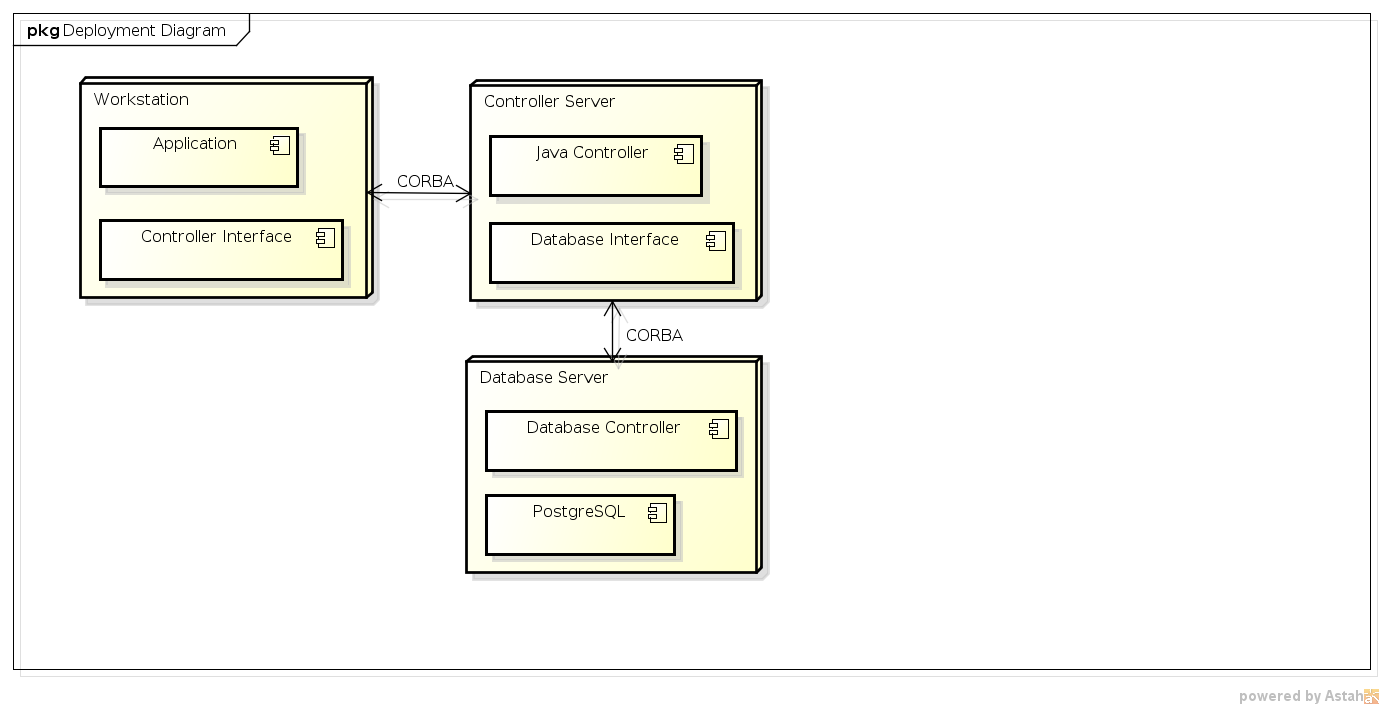
\includegraphics[width=14cm]{images/DeploymentDiagram.png}
				\label{Diagrama-Deployment}
				\fonte{Acervo do autor}
		}}
	\end{figure}

\subsection{Diagrama de Classe}
	As classes que compõem o sistema, bem como as relações entre cada classe, são apresentadas
	na Figura \ref{Diagrama-Classe} e servem também para a modelagem do \textit{middleware}.
	
	As classes \textit{Transaction, Tag} e \textit{Period} servem para armazenamento e transição de informações, não apresentam nenhum método. O manuseio dos dados é executado pelas classes \textit{TagController} e \textit{PeriodController}, que por sua vez não necessitam de atributos.
	
	\begin{figure}[!htb]
		\caption{Diagrama de Classe}
		{\parbox{6cm}{
				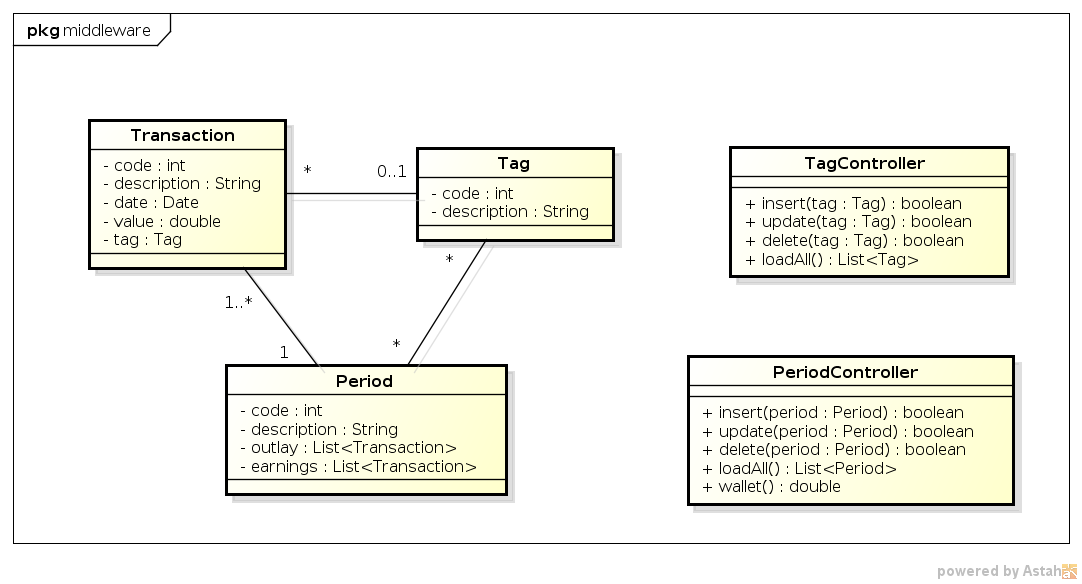
\includegraphics[width=10cm]{images/ClassDiagram.png}
				\label{Diagrama-Classe}
				\fonte{Acervo do autor}
		}}
	\end{figure}

\subsection{Diagramas de Sequência}
	Os diagramas de sequência das figuras \ref{SeqTag}, \ref{SeqPeriod} e \ref{SeqTransaction} apresentam os fluxos básicos da aplicação. A partir deles é possível conhecer as principais funções do sistema.
	
	O processo de criação de \textit{Tag} está apresentado na Figura \ref{SeqTag} e consiste na criação por parte do usuário de uma nova instância do modelo \textit{Tag}, preenchimento dos seus dados e envio ao controlador para validação, em caso positivo é solicitado ao servidor de persistência para que a nova \textit{Tag} seja salva e uma mensagem de sucesso é retornada ao usuário.
	
	\begin{figure}[!htb]
		\caption{Diagrama de Sequência de adição de \textit{tag}}
		{\parbox{6cm}{
				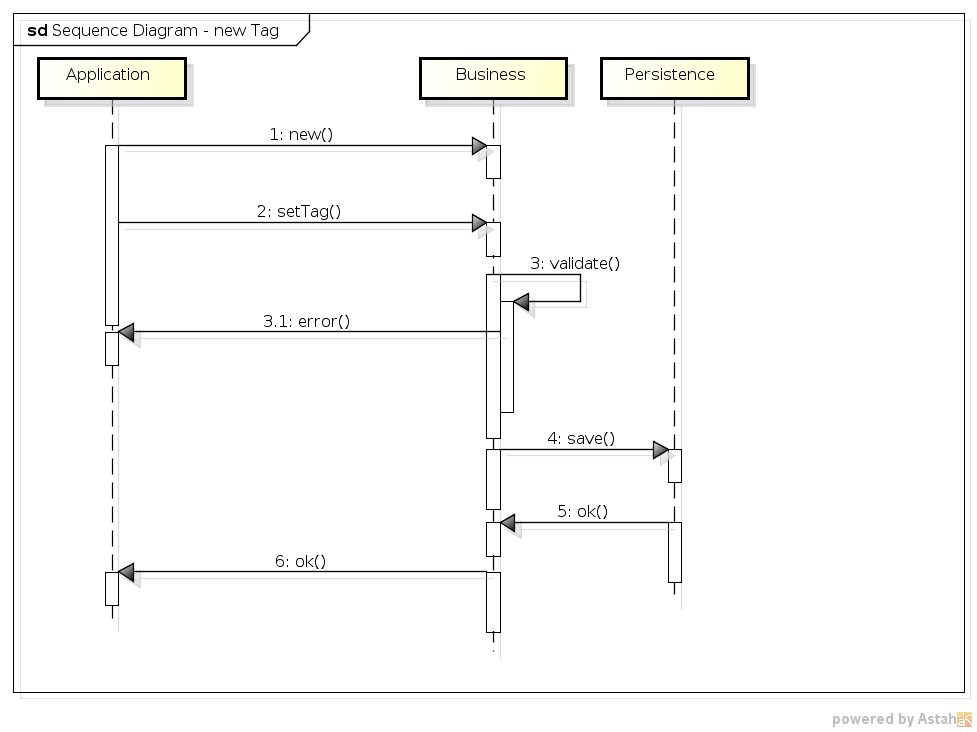
\includegraphics[width=10cm]{images/SequenceDiagramNewTag.png}
				\label{SeqTag}
				\fonte{Acervo do autor}
		}}
	\end{figure}

	A Figura \ref{SeqPeriod} apresenta a criação de um novo período no sistema, este receberá uma descrição e abrirá uma nova lista de transações. O servidor de controle validará as informações e enviará a persistência para que o novo período seja salvo.

	\begin{figure}[!htb]
		\caption{Diagrama de Sequência de adição de Período}
		{\parbox{6cm}{
				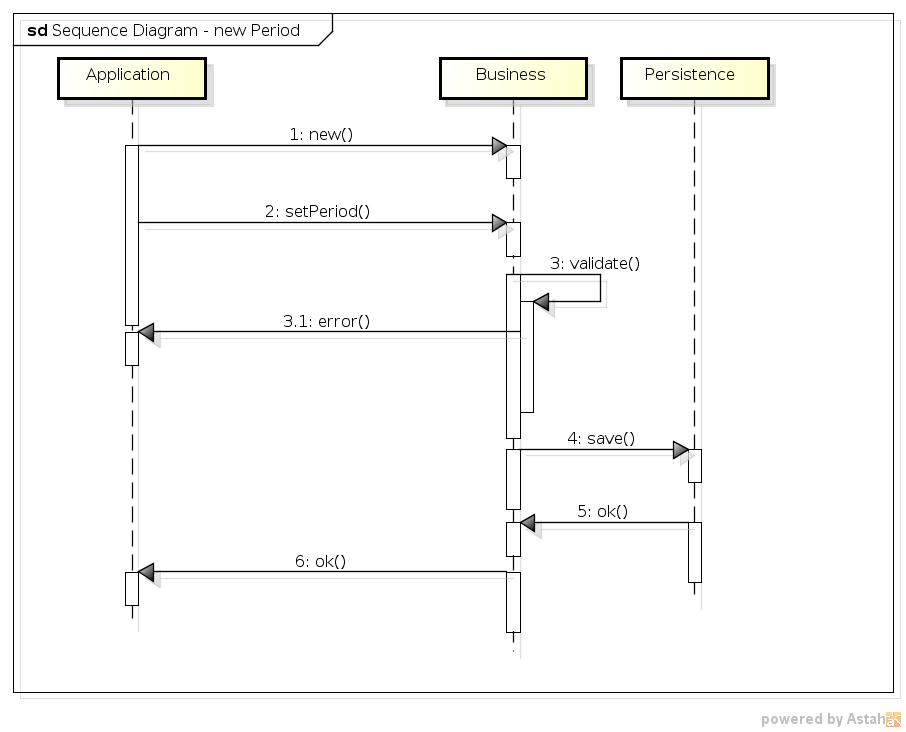
\includegraphics[width=10cm]{images/SequenceDiagramNewPeriod.png}
				\label{SeqPeriod}
				\fonte{Acervo do autor}
		}}
	\end{figure}

	Após ter um período criado é possível adicionar transações de ganhos ou despesas a ele. Uma nova transação deverá ter uma descrição, valor e data, podendo ser atribuído uma \textit{tag}. Ao finalizar o cadastro a aplicação repassa a solicitação para o servidor de controle, que valida as informações e envia para persistência. Sempre que o processo ocorrer corretamente a lista de transações é atualizada, bem como o valor na carteira. Este fluxo está presente da Figura \ref{SeqTransaction}.
	
	\begin{figure}[!htb]
		\caption{Diagrama de Sequência de adição de transação}
		{\parbox{6cm}{
				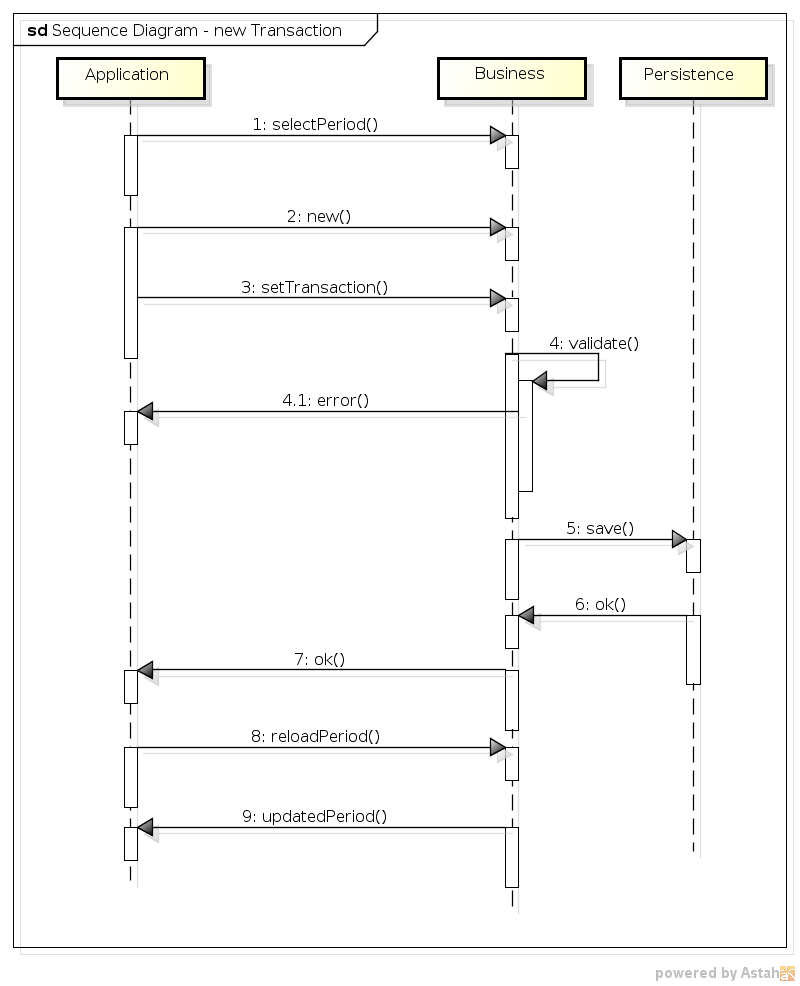
\includegraphics[width=10cm]{images/SequenceDiagramNewTransaction.png}
				\label{SeqTransaction}
				\fonte{Acervo do autor}
		}}
	\end{figure}

%DESENVOLVIMENTO
\chapter{DESENVOLVIMENTO}

\section{Exposição do Tema ou Matéria}



% 
%--------- FIM DESENVOLVIMENTO------------
%

%CONCLUSÃO
%\chapter{CONCLUSÃO}

As conclusões devem responder às questões da pesquisa, em relação aos objetivos e hipóteses. Devem ser breves podendo apresentar recomendações e sugestões para trabalhos futuros.  

% ----------------------------------------------------------
% ELEMENTOS PÓS-TEXTUAIS
% ----------------------------------------------------------
%\postextual

% ----------------------------------------------------------
% Referências bibliográficas
% ----------------------------------------------------------

\bibliography{referencias}
\nocite{Nelson-VM-Migration}
\nocite{Phi-Load-Balance}
\nocite{Khandekar}
%Apêndices
% \begin{apendicesenv}

\chapter{Título do Apêndice A}

Arquivos confeccionados pelo autor do trabalho e que não se encaixam no texto.

 Ex: Deduções matemáticas, dimensionamentos extensos e algoritmos.

\end{apendicesenv}

%Anexos
% \begin{anexosenv}
\chapter{Título do Anexo A}
\label{anexoA}

Arquivos não confeccionados pelo autor do trabalho.


\end{anexosenv}

%---------------------------------------------------------------------
% INDICE REMISSIVO
%---------------------------------------------------------------------
% \printindex
\end{document}